\subsubsection{Insertion Latency}
\label{s:meas_insert}

\begin{figure*}[!tb]
\centering
\subfloat[burst size 100, same priority\label{fig:bcm_burst_100_same_pri}]
  {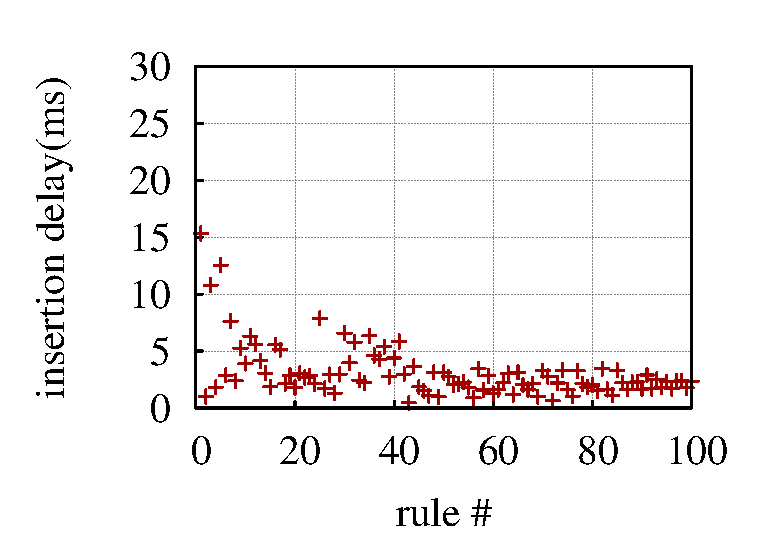
\includegraphics[width=.24\linewidth]{./figs/jan27_bcm_add_same_burst_100.eps}}\hfill
\subfloat[burst size 200, same priority\label{fig:bcm_burst_200_same_pri}]
  {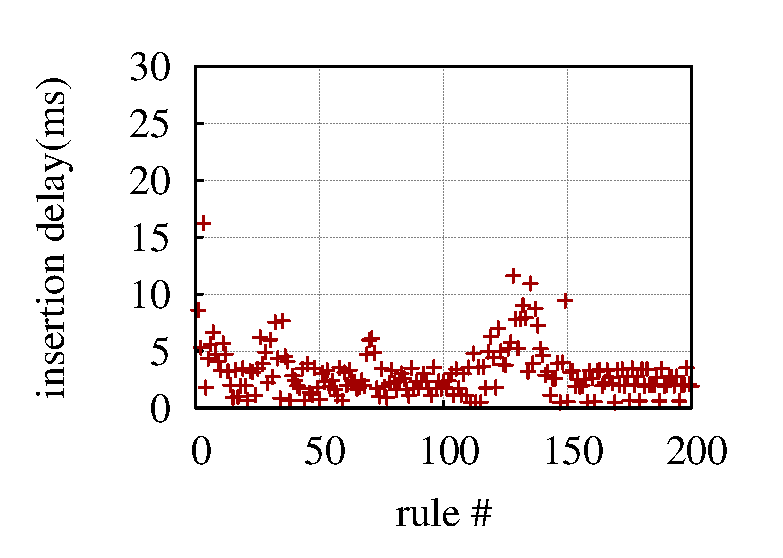
\includegraphics[width=.24\linewidth]{./figs/jan27_bcm_add_same_burst_200.eps}}\hfill
\subfloat[burst size 100, incr. priority\label{fig:bcm_burst_100_incr_pri}]
  {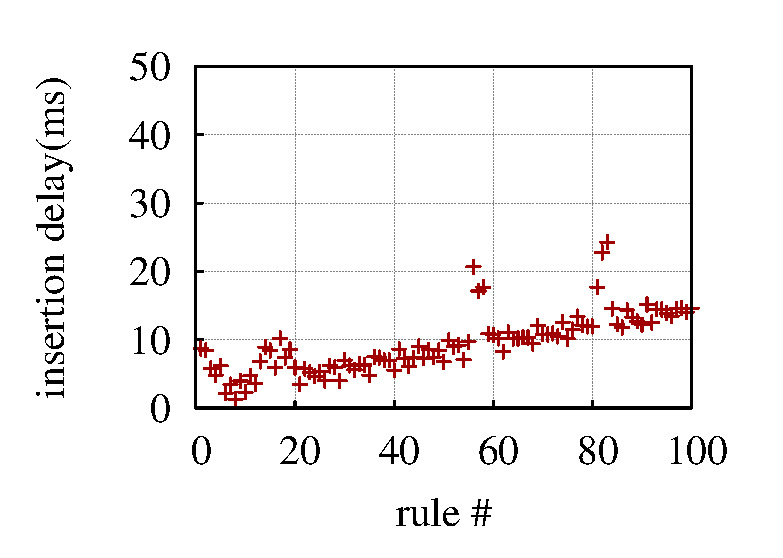
\includegraphics[width=.24\linewidth]{./figs/jan27_bcm_add_incr_burst_100.eps}}\hfill
\subfloat[burst size 200, incr. priority\label{fig:bcm_burst_200_incr_pri}]
  {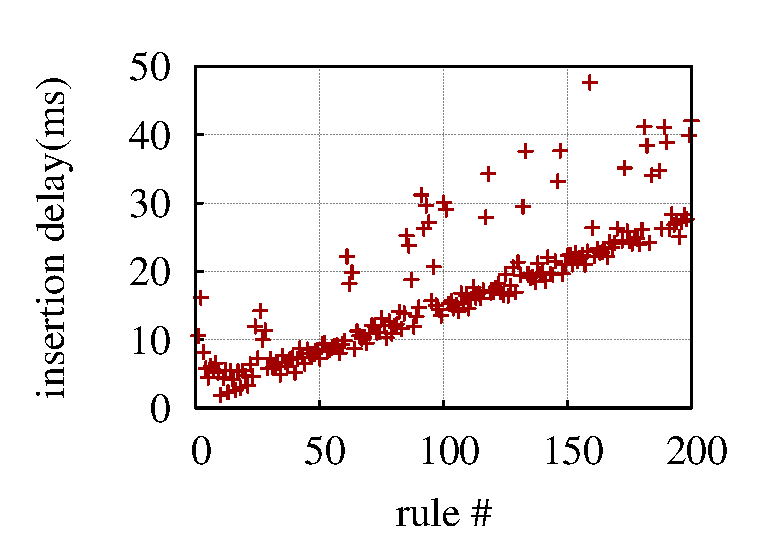
\includegraphics[width=.24\linewidth]{./figs/jan27_bcm_add_incr_burst_200.eps}}
\topcompactcaption{{\bf \BroadcomOne} priority per-rule {\bf insert} latency}
\label{fig:priority-broadcom-insert}
\end{figure*}


We first examine how different rule workloads impact insertion latency. We
insert a burst of $B$ rules: $r_1,\cdots,r_B$. Let $T(r_i)$ be the time we
observe the first packet matching $r_i$ emerging from the output port
specified in the rule. We define per-rule insertion latency as $T(r_i)-T(r_{i-1})$.  

%We conduct a variety of tests to examine how different patterns of
%rule workloads impact insertion latency. In almost all experiments, we
%install a burst of rules. Let us denote these rules
%in a sequence as $r_1, r_2,\cdots,r_i,\cdots, r_B$. Denote $T(r_i)$ as the time we
%observe the first packet matching $r_i$ emerging from the intended port of the rule
%action. We define insertion latency as $T(r_i)-T(r_i-1)$.  

\minisection{Rule Complexity} 
To understand the impact of rule complexity (i.e., the number of header 
fields specified in a rule), we install bursts of rules that specify either
2, 8, or 12 fields. In particular, we specify destination IP and EtherType
(others wilcarded) in the 2-field case; input port, EtherType, source and
destination IPs, ToS, protocol, and source and destination ports in the
8-field case; and all supported header fields in the 12-field (exact match)
case. We use a burst size of 100 and all rules have the same priority.

%To understand the impact of rule complexity (i.e., the number and type of
%matching fields specified in a rule), we conduct three different
%experiments with a fixed burst size ($B$ = 100) and priority but the rules
%having different matching fields. In the first experiment, all the rules in a
%burst only have only 2 match fields (others wildcarded), in the second
%experiment all the rules have 8 match fields (others wildcarded), and in the
%third experiment the rules have all the 12 match fields set (exact match).
%For the 2-match field experiment, we specified the destination IP and
%EtherType as the matching fields and for the 8-match field experiment we
%specified all the matching fields except source mac, destination mac, vlan id
%and vlan priority.  

We find that rule complexity {\em does not} impact insertion latency. The
mean per-rule insertion delay for 2-field, 8-field, and exact
match cases is 3.31ms, 3.44ms, and 3.26ms, respectively, for \BroadcomOne.
Similarly, the mean per-rule insertion delay for \BroadcomThree is $\approx$ 
1 ms irrespective of the number of fields. 
All experiments that follow use rules with 2 fields.

%\emph{\BroadcomOne:} The mean per rule insertion delay is 3.31, 3.44 and 3.26 ms for 2-match field, 8-match field and exact match experiments respectively. This indicates that the insertion time does not vary with rule complexity on \BroadcomOne.

%\emph{\BroadcomThree:} 
%We observed that when a burst of rules is inserted, the \BroadcomThree firmware organizes the rules into batches. 
%Each batch has a size of about 50 rules and a single batch of rules is scheduled for insertion every 4 seconds. 
%This effect adds significant delay (4 seconds) between processing of two consecutive batches.
%This can be attributed to the inefficent firmware implementation which is still in its early stage of development. 
%We assume that the batching effect is due to unoptimized firmware and will be fixed in the near future. 
%Hence, we only consider the batch completion time when discussing insertion time on \BroadcomThree.  


%For 2-field, 8-field and exact match experiments the mean batch completion time 
 %(mean per rule insertion time) 
%is about 47 ms, 45 ms, 51 ms. This indicates that the %insertion time is not dependent on rule complexity on %\BroadcomThree neither. 

\minisection{Table occupancy} To understand the impact of table occupancy, we
insert a burst of $B$ rules into a switch that already has $S$ rules
installed. All $B+S$ rules have the same priority. We fix $B$ and
vary $S$, ensuring $B+S$ rules can be accommodated in each switch's hardware
table.

%\li{TODO: Keqiang, please add corresponding numbers in text for Broadcom and
%  Intel. } 

We find that the flow table occupancy {\em
does not} impact the insertion operation if all rules have the same priority.
Taking $B=400$ as an example, the mean per-rule insertion delay is 3.14ms, 
1.09ms, and 1.11ms, and the standard
deviation is 2.14ms, 1.24ms, and 0.18ms for \BroadcomOne, \BroadcomThree,
and \Intel, respectively, regardless of the value of $S$. 
%However, flow table occupany has an indirect impact through priority which
%we will cover next.  investigate in Section~\ref{sec:priority}. 

\minisection{Rule priority} To understand the effect of rule priority on the
insertion operations, we conducted three different experiments each covering
different patterns of priorities. In each, we insert a burst of $B$ rules
into an empty table ($S=0$); we vary $B$. In the {\em same priority}
experiment, all rules have the same priority. In the {\em increasing} and
{\em decreasing priority} experiments, each rule has a different priority and
the rules are inserted in increasing/decreasing priority order, respectively. 

\emph{\BroadcomOne, same priority.} 
%We experimented with several values of $B$. 
Representative results for $B=100$ and $B=200$ are shown in
\figsref{fig:bcm_burst_100_same_pri}{fig:bcm_burst_200_same_pri}, respectively. In both
cases, we see that the per-rule insertion delay is similar: with
medians of 3.12ms and 3.02ms, and standard deviations of 1.70ms and 2.60ms, 
for $B=100$ and $B=200$, respectively. 
% insert $B=100$ rules in the
% switch. As shown in Figure~\ref{fig:priority-broadcom-insert}-a, the per rule
% insertion delay among the 100 rules are similar with median xx ms and standard
% deviation xx. As shown in Figure~\ref{fig:priority-broadcom-insert}-b, the
% insertion delay for burst size 200 has a median xx ms and standard deviation
% xx. We also perform other burst sizes. The results are similar.
We conclude that same priority rule insertion delay does not vary with burst size on \BroadcomOne.

\emph{\BroadcomOne, increasing priority.}
\figref{fig:bcm_burst_100_incr_pri} shows the result for
$B=100$. We note that the per-rule insertion delay actually {\em
  increases linearly} with the number of
rules inserted. \figref{fig:bcm_burst_200_incr_pri}
shows the result for $B=200$; we see that the slope stays the same as
$B=100$. Compared with the same priority experiment, the average per-rule
delay is much larger: 9.47ms (17.66ms) vs 3.12ms (3.02ms), for $B=100$ (200). 
Results for other values of $B$ are qualitatively similar. 
%li: does not parse, rewrite
%Thus, the latency experienced
%by a rule can be impacted by when the priorities of rules inserted
%immediately ahead of it are lower.
The TCAM in this switch stores high priority rules at low (preferred)
memory addresses. Thus, each rule inserted in this experiment
displaces all prior rules!

\emph{\BroadcomOne, decreasing priority.} 
We also perform decreasing priority insertion (not shown). The average 
per-rule insertion delays for $B=100$ and $B=200$ are 8.19ms and 15.5ms, respectively. We observe that the burst of $B$ rules is divided into a number 
of groups, and each group is reordered and inserted in the TCAM in order of increasing priority. 
%\aditya{the following is weird} We have been
%working with Broadcom in our measurements. The feedback is that Broadcom has not
%optimized their software to handle rule priority optimally in all cases.
This indicates that \BroadcomOne firmware reorders the rules and prefers
increasing priority insertion. 
%\keqhe{The average per-rule insertion delays for $B=100, B=200$ with decreasing priority are 8.19ms and 15.5ms respectively.}\aaron{We need some numbers here so we can
%compare against them in the \BroadcomThree results below.}

\iffalse
\emph{\BroadcomThree.} 
In \BroadcomThree we observed that when a burst of rules is inserted, 
the firmware organizes the rules into batches. 
Each batch has a size of about 50 rules and a single batch of rules is scheduled for insertion every 4 seconds. 
This effect adds significant delay (4 seconds) between processing of two consecutive batches. 
This can be attributed to the inefficent firmware implementation which is still in its early stage of development. 
We assume that the batching effect is due to unoptimized firmware and will be fixed in the near future. Hence, 
we ignore the inter-batch processing delays and only consider the batch completion time.  
\sourav {I am not sure if this a correct way of addresing this. 
What should we say here? The reasons for this batching effect are still unknown}
\fi
\emph{\BroadcomThree, same priority.} 
The mean per-rule insertion
delay is 1.09ms (1.08ms) for $B=100$ (200). Thus, similar to \BroadcomOne,
the rule insertion time does not vary with burst size when all rules are of
the same priority. 

\emph{\BroadcomThree, increasing priority.} 
The average per-rule insertion delay is much 
larger: 7.75ms (16.81ms) for $B = 100$ (200). This is similar to our findings
for \BroadcomOne, affirming that TCAM organization requirements, not software
implementation issues, are the primary cause.
%This shows that the TCAM organization in case of \BroadcomThree is similar to that of \BroadcomOne where high priority rules are stored at low memory addresses. 


%the mean completion time (per rule insertion time)  for 1st, 2nd, 3rd and 4th batch is 284 (5.68), 589 (11.78), 1192 (23.84) and 2022 (40.44) ms respectively which is significantly higher than the same priority completion time. This shows that the TCAM organization in case of \BroadcomThree is similar to that of \BroadcomOne where high priority rules are stored at low memory addresses. 

\emph{\BroadcomThree, decreasing priority.} 
The per-rule delay is similar to that of
same priority insertion: $\approx 1$ms. This contrasts with
\BroadcomOne, where decreasing priority insertion increases with the
number of rules inserted---average of 8.19ms (15.5ms) for $B=100$ (200). 
Hence the \BroadcomThree firmware has been better optimized to handle 
decreasing priority rule insertions.
%This shows that \BroadcomThree optimizes decreasing priority rule insertions 
%efficiently unlike \BroadcomOne. \aaron{Fix the preceding sentence after we
%have numbers in \BroadcomOne decreasing priority above.}
%In case of increasing priority experiment the per rule insertion delay increases with increase in burst size. Compared with the same priority experiment the average per rule insertion delay in this case is larger: ??? (???) vs ??? (???) for B = 100 (200). However for decreasing priority experiment,  the delay is much smaller than  \BroadcomOne and does not vary with the burst size. The mean delay for   
%for B = 100 and 200 is ??? and ??? ms respectively. This shows that while the 
%\BroadcomThree firmware is more optimized than \BroadcomOne firmware  for decreasing priority rule insertion, the delays are still large for increasing priority rule insertion because of the way TCAM organizes rules in the table(high priority at low memory addresses).

% We next show our measurement results on Intel. 

\begin{figure}[!tb]
\centering
%\subfloat[burst size 800, same priority.\label{fig:intel_burst_800_same_pri}]
 %{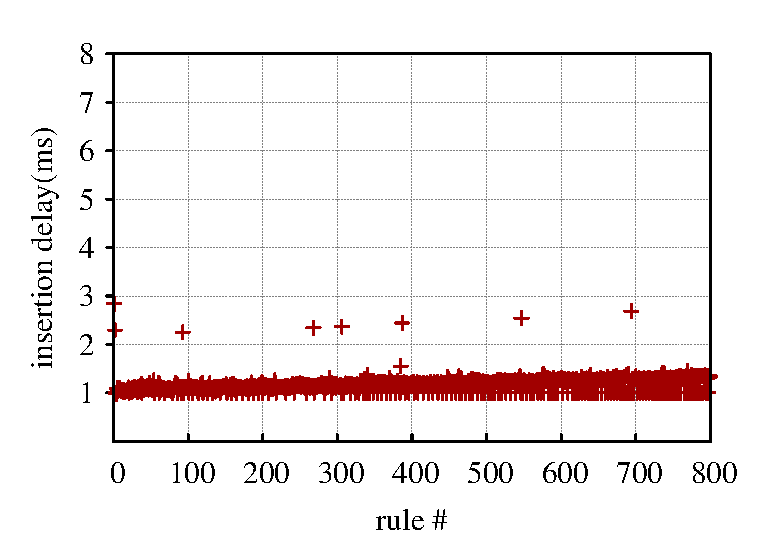
\includegraphics[width=.33\linewidth]{./figs/jan27_intel_same_burst_800.eps}}\hfill
%\subfloat[burst size 200, same priority.\label{fig:intel_burst_200_same_pri}]
%  {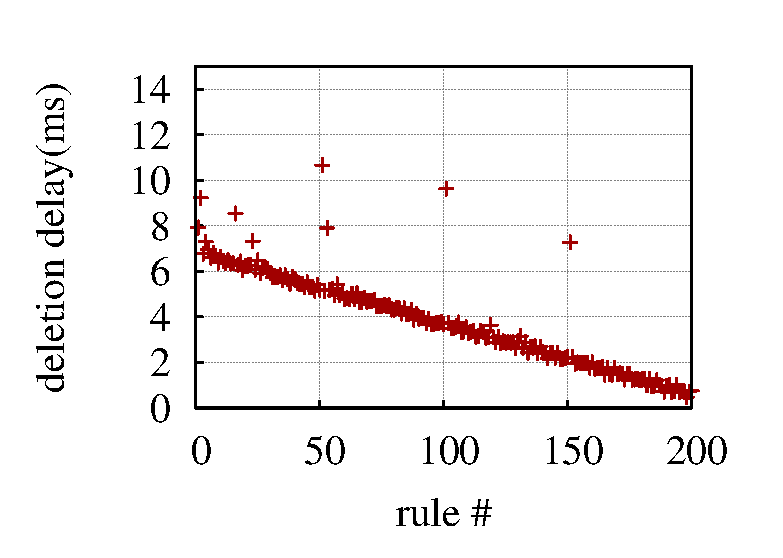
\includegraphics[width=.24\linewidth]{./figs/jan27_intel_same_burst_200.eps}}\hfill
\subfloat[burst size 800, incr. priority\label{fig:intel_burst_800_incr_pri}]
  {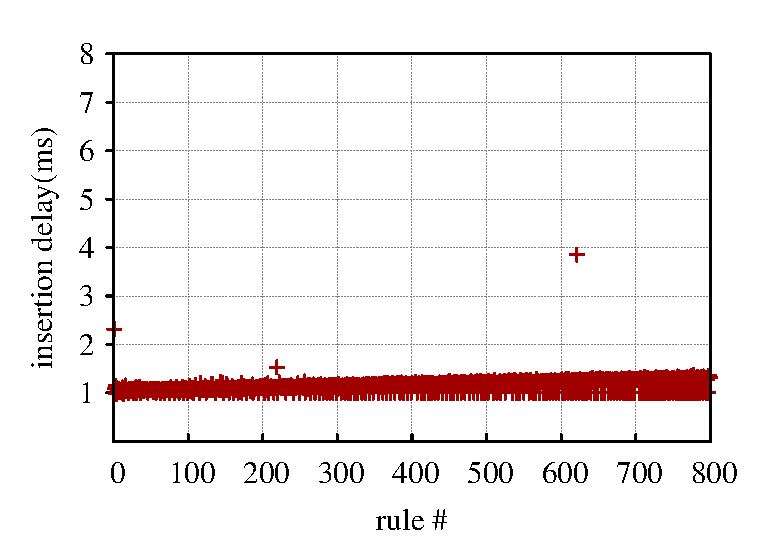
\includegraphics[width=.49\linewidth]{./figs/jan27_intel_incr_burst_800.eps}}\hfill
\subfloat[burst size 800, decr. priority\label{fig:intel_burst_800_decr_pri}]
 {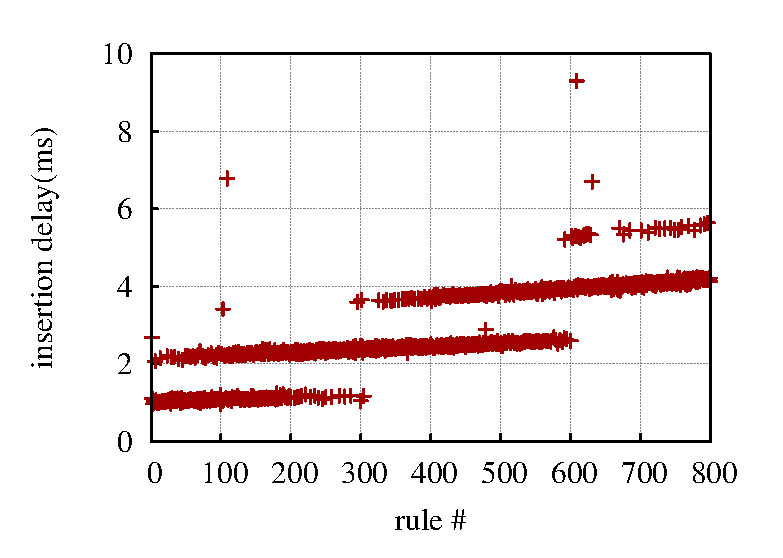
\includegraphics[width=.49\linewidth]{figs/jan27_intel_empty_800L_decr_delta.eps}}
%\subfloat[burst size 200, decreasing priority.\label{fig:intel_burst_200_incr_pri}]
%  {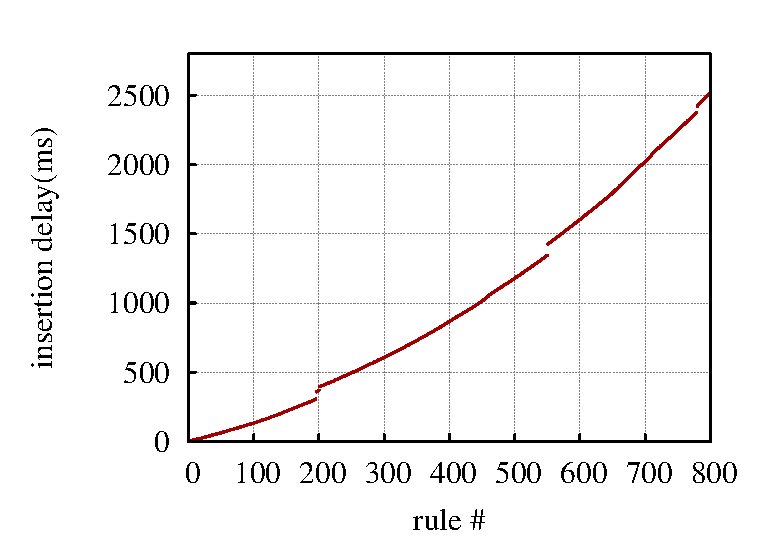
\includegraphics[width=.24\linewidth]{figs/jan27_intel_3200H_800L_decr_real.eps}
\topcompactcaption{{\bf Intel} priority per-rule {\bf insert}
%: (a) burst size
%  100, same priority (b) burst size 200, same priority (c) burst size 100,
%  increasing priority (d) burst size 200, increasing priority {\bf TODO: (e) burst size
%  100, decreasing priority (f) burst size 200, decreasing priority; SHOW the
%  priority effect}
} 
\label{fig:priority-intel-insert}
\end{figure}

\emph{\Intel, same priority.} %Figure~\ref{fig:priority-intel-insert}(a)
For $B=800$ on \Intel\footnote{We present results for a larger value of $B$ 
because the flowtable size on \Intel is larger (\tabref{switch_para}).} we see that the per-rule
insertion delay is similar across the 800 rules, with a median of 1.17ms and
standard deviation of 0.16ms (not shown). 
% \aaron{It is odd to show results for B=100 and B=200 for \BroadcomOne, but B=800 for Intel? Do we have higher values of B (e.g., B=600) for \BroadcomOne, so we can use the same B value(e.g., B=600) for both?} 
The results for other values of $B$ are similar. Thus, similar to
\BroadcomOne and \BroadcomThree, same priority rule insertion delay does not
vary with burst size on \Intel. 
%The result for $B=200$ in
%Figure~\ref{fig:priority-intel-insert}(b) shows a similar trend with a
%median delay of xx ms and a standard deviation of
%xx. \aditya{the two sets of lines is interesting and merits
%  discussion!} Thus, similar to Broadcom, same priority rule insertion
%delay does not vary with burst size on Intel.
% we see that the
% same-priority rules isinsertion of a higher priority rule is totally unimpacted by the lower
% priority rules inserted immediately ahead of it. 
% priority rule insertion delay does not vary with burst size on Intel,
% similar to Broadcom.

\emph{\Intel, increasing priority.} %\aditya{graphs for this are missing}
\figref{fig:intel_burst_800_incr_pri} shows per-rule latencies for
$B=800$. \emph{Surprisingly}, in contrast with \BroadcomOne and
\BroadcomThree, the per rule
insertion delay among the rules is more or less the same, with a
median of 1.18ms and a standard deviation of 1.08ms.  We see similar
results for other values of $B$. This shows that the \Intel TCAM architecture 
is fundamentally different from \Broadcom. 
%\aditya{is this a hardware  difference? can it not be SDK?} 
%li: yes, hardware 
Rules are ordered in \Intel's TCAM such that higher priority rule insertion
does not displace existing low priority rules. 
%\aditya{why are we talking about displacement here? we did not mention this for
%broadcom} 

\emph{\Intel, decreasing priority.} %\aditya{graphs for this are missing} 
%The insertion delay increases for decreasing priority insertion.  Rule arrangement in
%  TCAM is such that low priority rule insertion causes displacement of high
%  priority rules. \aditya{this does not appear to be true}
\figref{fig:intel_burst_800_decr_pri} shows per-rule insertion latencies for
$B=800$. We see two effects: (1) the latencies alternate between two modes at any
given time, and (2) a step-function effect after every 300 or so
rules. 

A likely explanation for the former is bus buffering. Since rule insertion is 
part  of the switch's control path, it is not really optimized for latency.
The latter effect can be explained as follows: Examining the \Intel switch architecture, we
find that it has 24 slices, $A_1\ldots A_{24}$, and each slice holds 300
flow entries. There exists a consumption order (low-priority first) across
all slices.  Slice $A_i$ stores the $i^{th}$ lowest priority rule group. If
rules are inserted in decreasing priority, $A_1$ is consumed first until it
becomes full. When the next low priority rule is inserted, this causes one
rule to be displaced from $A_1$ to $A_2$.  This happens for each of the next
300 rules, after which cascaded displacements happen: $A_1 \rightarrow A_2
\rightarrow A_3$, and so on. We confirmed this with \Intel.
%\aditya{we dont have a good explanation for 1}

% ; then $A_2$ starts to be consumed. However, due to the
% decreasing order, 299 existing rules in $A_1$ must be moved into $A_2$, and
% then a new inserted rule will be written into slice $A_1$ until it
% becomes full.
%full, and so on. 


%We suspect some rules trigger
%TCAM reordering and some do not. This results in an ON and OFF process that adds
%delay if the process is on.  
%\aditya{the following is weird} We have been working with Intel closely on our
%measurements. The feedback we got 
%from Intel is that their switch firmware has not been optimized to handle rule
%priorities efficiently in all cases.
%\li{are the two modes strictly alternative? Even rule number mode 1, odd rule
%  number mode 2??}

\minisection{Priority and table occupancy combined effects} 
%Given our understanding of the impact of rule priority and table occupancy on
%per-rule insertion latency, we now study their combined impact. 
We now study the combined impact of rule priority and table occupancy.
We conduct two experiments: For the first experiment, the table starts with
$S$ high priority rules, and we insert $B$ low priority rules.  For the
second experiment, the priorities are inverted.
For both experiments, we measure the total time to install all rules in the
burst, $T(r_B)-T(r_1)$.
%burst rule insertion completion time;
%many applications depend on this the metric (\secref{s:apps}). 

\begin{figure}
\subfloat[insert low priority rules into\newline a table with high priority rules\label{fig:bcm_outbound_two_pri_high_low_burstB}]
  {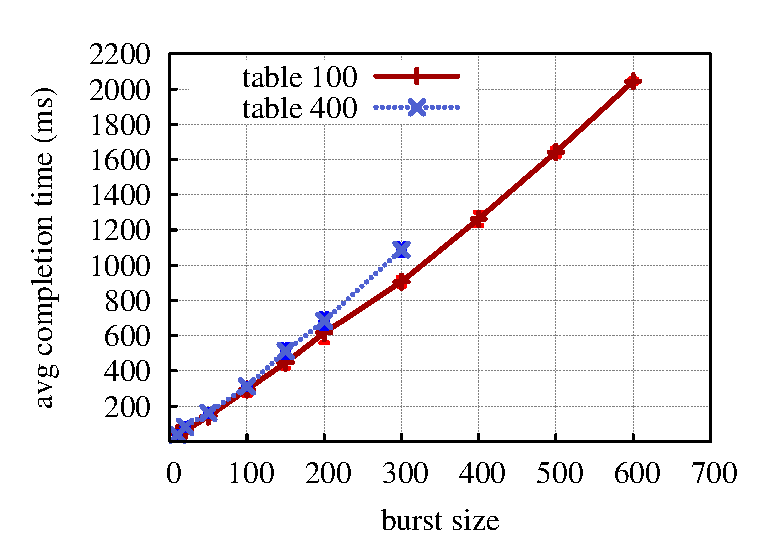
\includegraphics[width=.50\linewidth]{./figs/bcm_two_pri_high_low_burstB.eps}}\hfill
\subfloat[insert high priority rules into a table with low priority rules\label{fig:bcm_outbound_two_pri_low_high_burstB}]
  {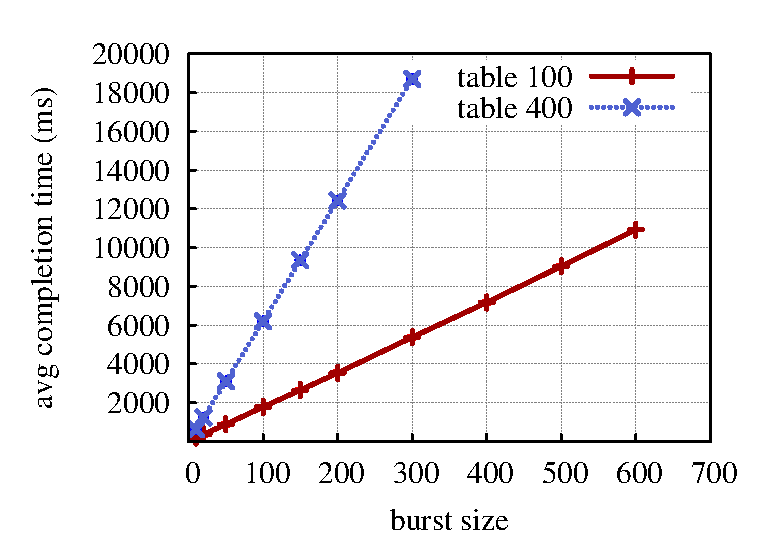
\includegraphics[width=.50\linewidth]{./figs/bcm_two_pri_low_high_burstB.eps}}
\compactcaption{Overall completion time on {\bf \BroadcomOne}.  Initial table occupancy is S high (low) priority rules; insert a burst of low (high) priority rules. Averaged over 5 runs. }
\label{fig:burst-completion-time}
\end{figure}

%We conduct two experiments. With $S$ rules in the table, we insert a burst of $B$ rules. 
%For the first experiment, $S$ has high priority and we insert the burst with low priority. 
%For the second experiment, if it is Broadcom (\BroadcomOne or \BroadcomThree), $S$ has low priority and we insert rules with high priority; if it is Intel, $S$ has high priority and we insert rules in {\em decreasing} priority.

For \BroadcomOne and \BroadcomThree, we expect that as long as the same
number of rules are displaced, the completion time for different values of
$S$ should be the same.
Indeed, from \figref{fig:bcm_outbound_two_pri_high_low_burstB} (for
\BroadcomOne), we see that even with 400 high priority rules in the
table, the insertion delay for the first experiment is no different from the
setting with only 100 high priority rules in the table. In contrast, in
\figref{fig:bcm_outbound_two_pri_low_high_burstB}, newly inserted high
priority rules will displace low priority rules in the table, so when
$S=400$ the completion time is about 3x higher than $S=100$. 
\iffalse
\begin{figure}[!tb]
\centering
\subfloat[decreasing priority\label{fig:intel_burst_100_incr_pri_1}]
  {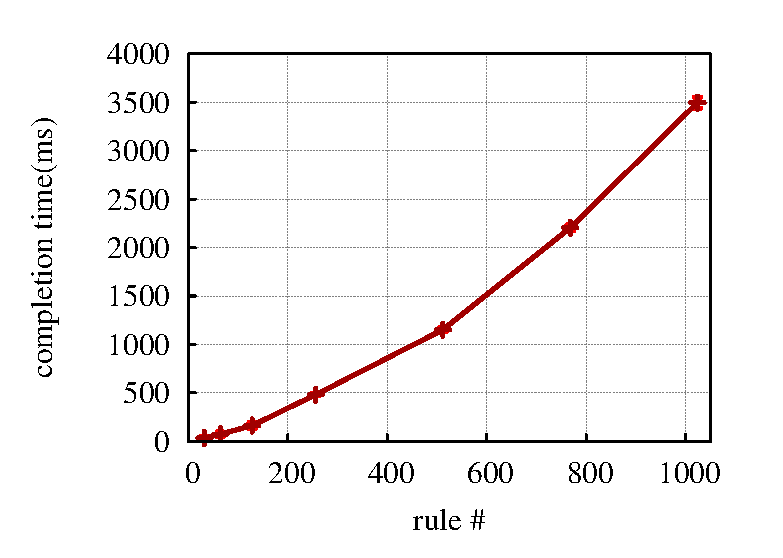
\includegraphics[width=.5\linewidth]{./figs/jan27_intel_decr_burst_size_effect.eps}}\hfill\caption{{\bf Intel} overall completion time} 
\label{fig:priority-intel-insert-more-results}
\end{figure}
\fi

%For \Intel, we also run the same two experiments as for Broadcom. 
For \Intel, the results are similar to same priority rule insertion.  This
indicates that \Intel optimizes for rule priority better than \BroadcomOne. 
\iffalse
When
we insert in decreasing priority
(\figref{fig:priority-intel-insert-more-results}) the completion time is
about 3.5 seconds, 3x higher than the case of same priority insertion.
\aaron{What is the point of these Intel results?}
\sourav{To show the worst case burst completion time on Intel since it does not have table occupancy effect. But now since the title has been changed from burst completion time to combined effect, I dont think this makes much sense here. }
 \fi
 
\minisection{Summary and root causes}
We observe that: (1) rule complexity does not affect insertion delay; (2)
same priority insertions in \BroadcomOne, \BroadcomThree, and \Intel are fast
and not affected by flow table occupancy; and (3) priority insertion patterns
can affect insertion delay very differently. For \Intel, increasing priority
insertion is similar to same priority insertion, but decreasing priority 
incurs much higher delay. For \BroadcomThree the behavior is inverted:  
decreasing priority insertion is similar to same priority insertion and increasing priority insertion incurs higher delay. For \BroadcomOne, 
insertions with different priority patterns are all much higher than
insertions with same priority. 

Key root causes for observed latencies are: (1) how rules are organized in the TCAM, and (2) the number of slices. {\em Both of these are intrinsically tied to switch hardware.} Even in the best case (\Intel), per-rule insertion latency of 1ms is higher than what native TCAM hardware can support (100M updates/s~\cite{estan:private}). Thus, in addition to the above two causes, there appears to be an {\em intrinsic switch software overhead} contributing to all latencies.

%\aditya{the following is weird} The feedbacks we got from both vendors are that
%their switch firmware has not been 
%optimized for rule priority. 

%\aditya{root causes is incomplete}

\iffalse
Each slice can hold 300 flow entries,
       Also, there exists a consumption order (low-priority first!) across all slices:
       A-slice: the lowest priority rule group, 
       B-slice: the second lowest priority rule group, ….etc  
       In such a case, if the flow rules are inserted in the decreasing priority order,
        A-slice will be first consumed until it becomes full.
        When A-slice is full, B-slice starts to be consumed.
        However, due to the decreasing order, 
       299 existing rules in A-slice must be moved into B-slice
       and then a new inserted rule will be written into A-slice.
       Until B-slice becomes full, and so on.

Based on a phone conversation:
The organization of the TCAM structure is 24 slices x 1024 lines x 36b. There is
also a remap stage between slices 12 and 13. For exact matching 12-tuple
conditions the lookup is split between the 2 halves (pre and post remap stage)
12 slices are used for each of the 12-tuple lookups. Under these conditions then
the OpenFlow table would be limited to 4 groups of 1K entries (4K total). 
If the Key used fewer tuples, or if it could be wild carded the maximum entries
in the TCAM block would be up to 24K. 
There is also an SRAM based Binary Search Tree (longest Prefix match). This is
organized as 4 slices x 16K entries x 32b. If this table is combined with the
TCAM then the maximum flow table size could be as large as 88K entries
(depending on Key size). 
\fi
% LocalWords:  Broadcom TODO Keqiang TCAM feedbacks
